\chapter{系统需求分析与总体架构设计}
这章会详细去介绍系统的功能需求分析和总体架构设计相关内容,一开始我们要深入分析系统需满足的功能需求,其中涵盖自然语言输入、语义理解、场景生成、仿真执行以及多样场景支持等关键方面,这些功能需求能给系统的设计提供明确方向和目标,接下来我们会阐述系统的总体架构设计,包含架构目标、设计原则、架构图展示以及模块间的数据流和交互机制,借助这些内容读者可对系统的整体设计有清晰了解,为后续章节各模块的具体设计与实现奠定基础。
\section{系统功能需求分析}
\subsection{高保真的驾驶测试需求}
在自动驾驶技术快速发展的背景下,自动驾驶系统的测试与验证变得特别重要,传统测试方法通常依靠手动构建场景,这种方式不仅耗费时间精力,而且难以覆盖复杂交通场景,为提高测试效率和覆盖度,本研究提出基于自然语言描述的三维智能驾驶场景生成系统,该系统能自动把用户输入的自然语言场景描述,转化为可执行的仿真场景并在CARLA仿真平台验证。

本系统的一大核心优势是能利用生成的智能驾驶场景,为自动驾驶技术提供高效且低成本的测试平台,传统人工构建测试场景的方法不仅耗时还费力,并且难以覆盖复杂的交通场景,使得测试成本高昂且效率非常低下,相比之下本系统借助自然语言输入和自动化场景生成技术,能够快速生成多样化的驾驶场景,显著提高了测试效率,用户只需通过简单的自然语言描述来输入,系统就可自动生成对应的三维智能驾驶场景,并在CARLA仿真平台上进行验证,这种自动化流程大大减少了人工干预,有效降低了测试成本,此外系统支持多种语义表达和场景组合,能够生成丰富的测试用例,满足不同阶段自动驾驶技术测试需求,通过这种方式本系统不仅能加速智能驾驶技术的开发和验证过程,还能为研究人员和工程师提供灵活可扩展的测试工具,推动智能驾驶技术不断发展。


\section{系统总体架构设计}
系统整体采用模块化分层设计,主要分为三个核心模块,每个模块分有几个子模块分别负责不同阶段的处理任务,构成完整的自然语言驱动智能驾驶场景生成流程:
\begin{figure}[H]
	\centering
	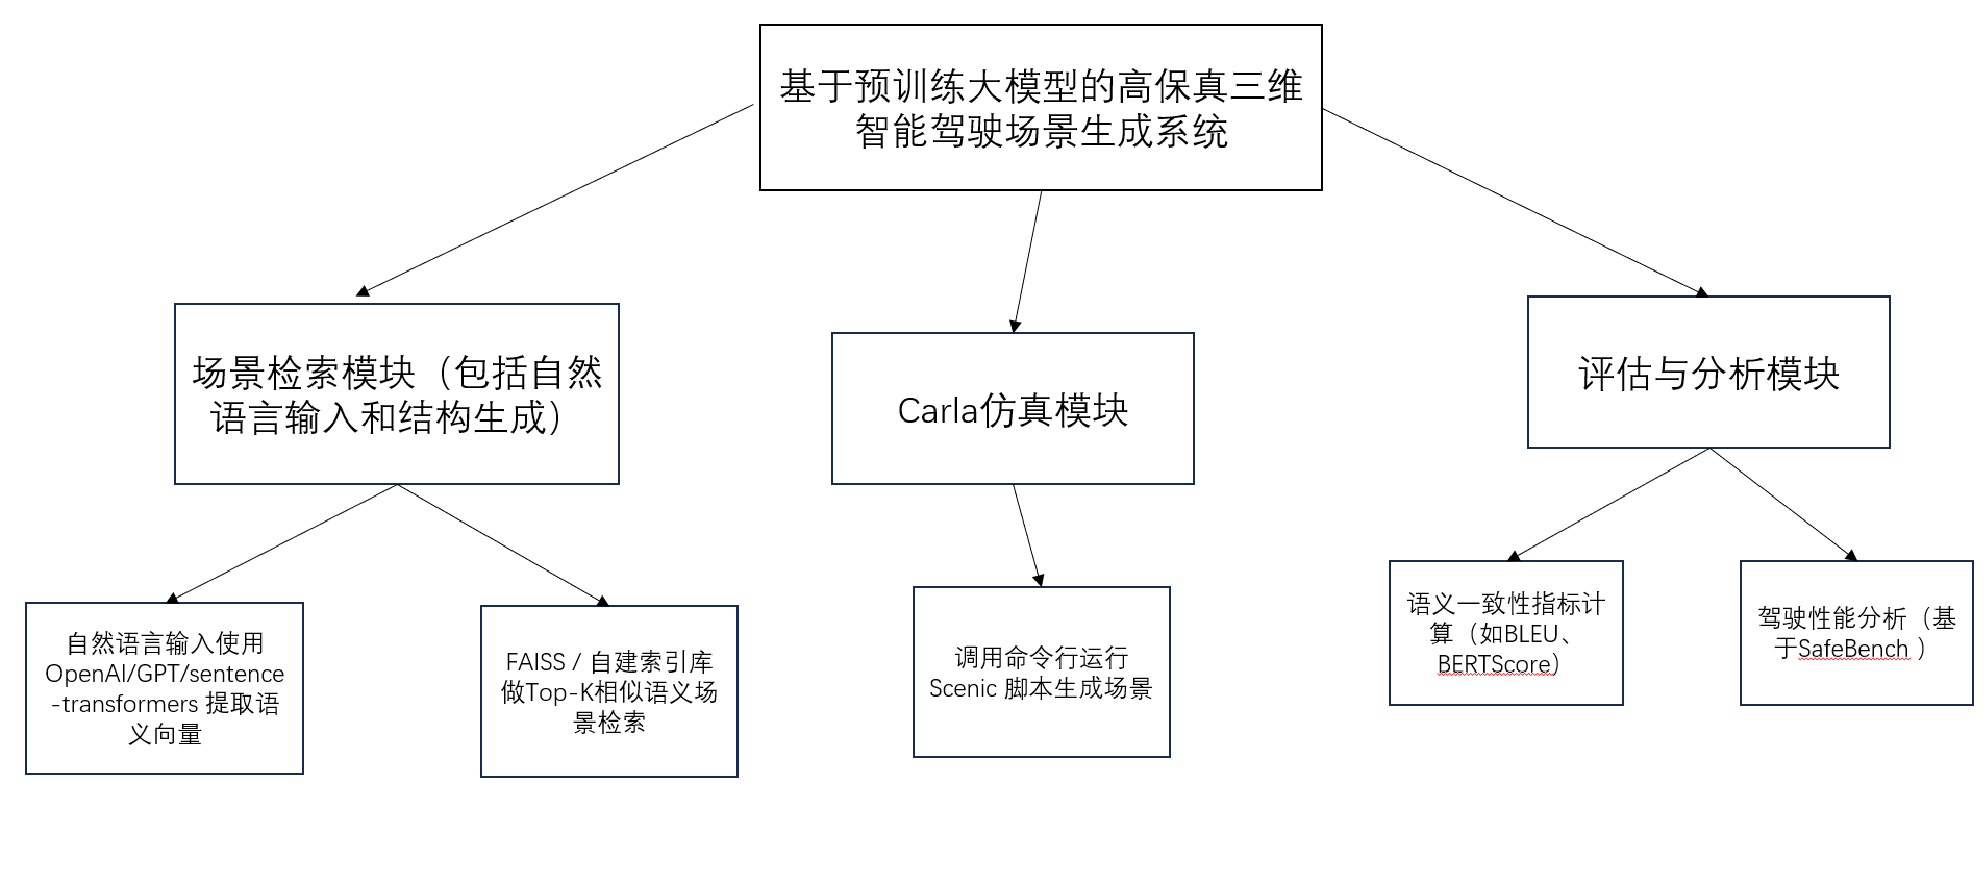
\includegraphics[width=1.0\textwidth]{images/系统架构图.pdf}
	\caption{系统架构}
	\label{fig:system-architecture}
\end{figure}
\subsection{自然语言输入模块}
考虑到需求分析的情况,本系统达成了支持用户以图形化界面或者命令行形式输入文字交通场景描述的功能,提供友好的人机交互体验来保证用户可方便输入各种场景描述,为实现这一目标,系统会采用PyQt5框架去构建图形化用户界面也就是GUI,以此确保界面具备简洁高效和跨平台兼容性的特点,PyQt5属于功能强大的Python GUI框架,能提供丰富控件与灵活布局选项,让开发者可设计出直观且易于使用的界面。

具体来说系统会遵循极简主义设计原则去除不必要复杂元素保证界面清晰直观,用户能够通过简单点击和输入操作完成场景描述输入无需复杂配置或学习,界面会提供清晰提示信息和操作指引来帮助用户快速上手使用,同时系统会优化输入流程减少用户操作步骤比如自动填充常见信息提供快捷输入选项提高输入效率,此外系统还支持用户保存输入的场景描述方便后续使用时快速调用和修改,为进一步提升用户体验系统可考虑引入智能提示功能依据用户输入内容实时推荐可能场景描述选项提高输入准确性和效率,总之系统自然语言场景输入功能以简洁高效为核心确保用户快速准确完成场景描述输入并享受流畅交互体验。

本系统在自然语言生成智能驾驶场景时采用 Sentence-T5-large 模型作为语义编码器,目的是从自然语言输入里提取语义向量并实现高效检索,Sentence-T5 是在 Google T5(Text-to-Text Transfer Transformer)模型基础上微调出来的句子级别语义模型,拥有对中文自然语言场景描述进行高质量语义建模的能力,T5 模型本质上是基于 Transformer 架构构建的,其核心部分是自注意力机制(Self-Attention),作用是捕捉输入序列中任意两个位置之间的依赖关系。

\subsection{结构生成模块}

结构生成模块作为本系统连接语义理解和仿真执行的核心环节,其主要任务是把语义检索得到的场景结构模板和自然语言输入内容进行融合,进而自动生成符合Scenic语法规范的结构化场景脚本也就是.scenic文件,该模块不但要对场景中的交通参与者及其属性进行表达,还需要描述它们的行为逻辑、空间约束以及触发机制,以此保证场景具备完整性、可执行性和可控性。

在实际进行实现的时候,系统维护着一组参数化 Scenic 模板脚本,模板里面预先设置了车辆、行人、道路、红绿灯等典型交通元素的结构框架与行为函数,要是用户输入“自车前方有行人突然横穿马路并停在车前”这样的内容,系统会匹配到“横穿 - 阻挡”场景模板,还会结合输入语义给其中的参数插槽自动赋值,像横穿速度、横穿位置、停止距离等。
如图:
\begin{figure}[H]
	\centering
	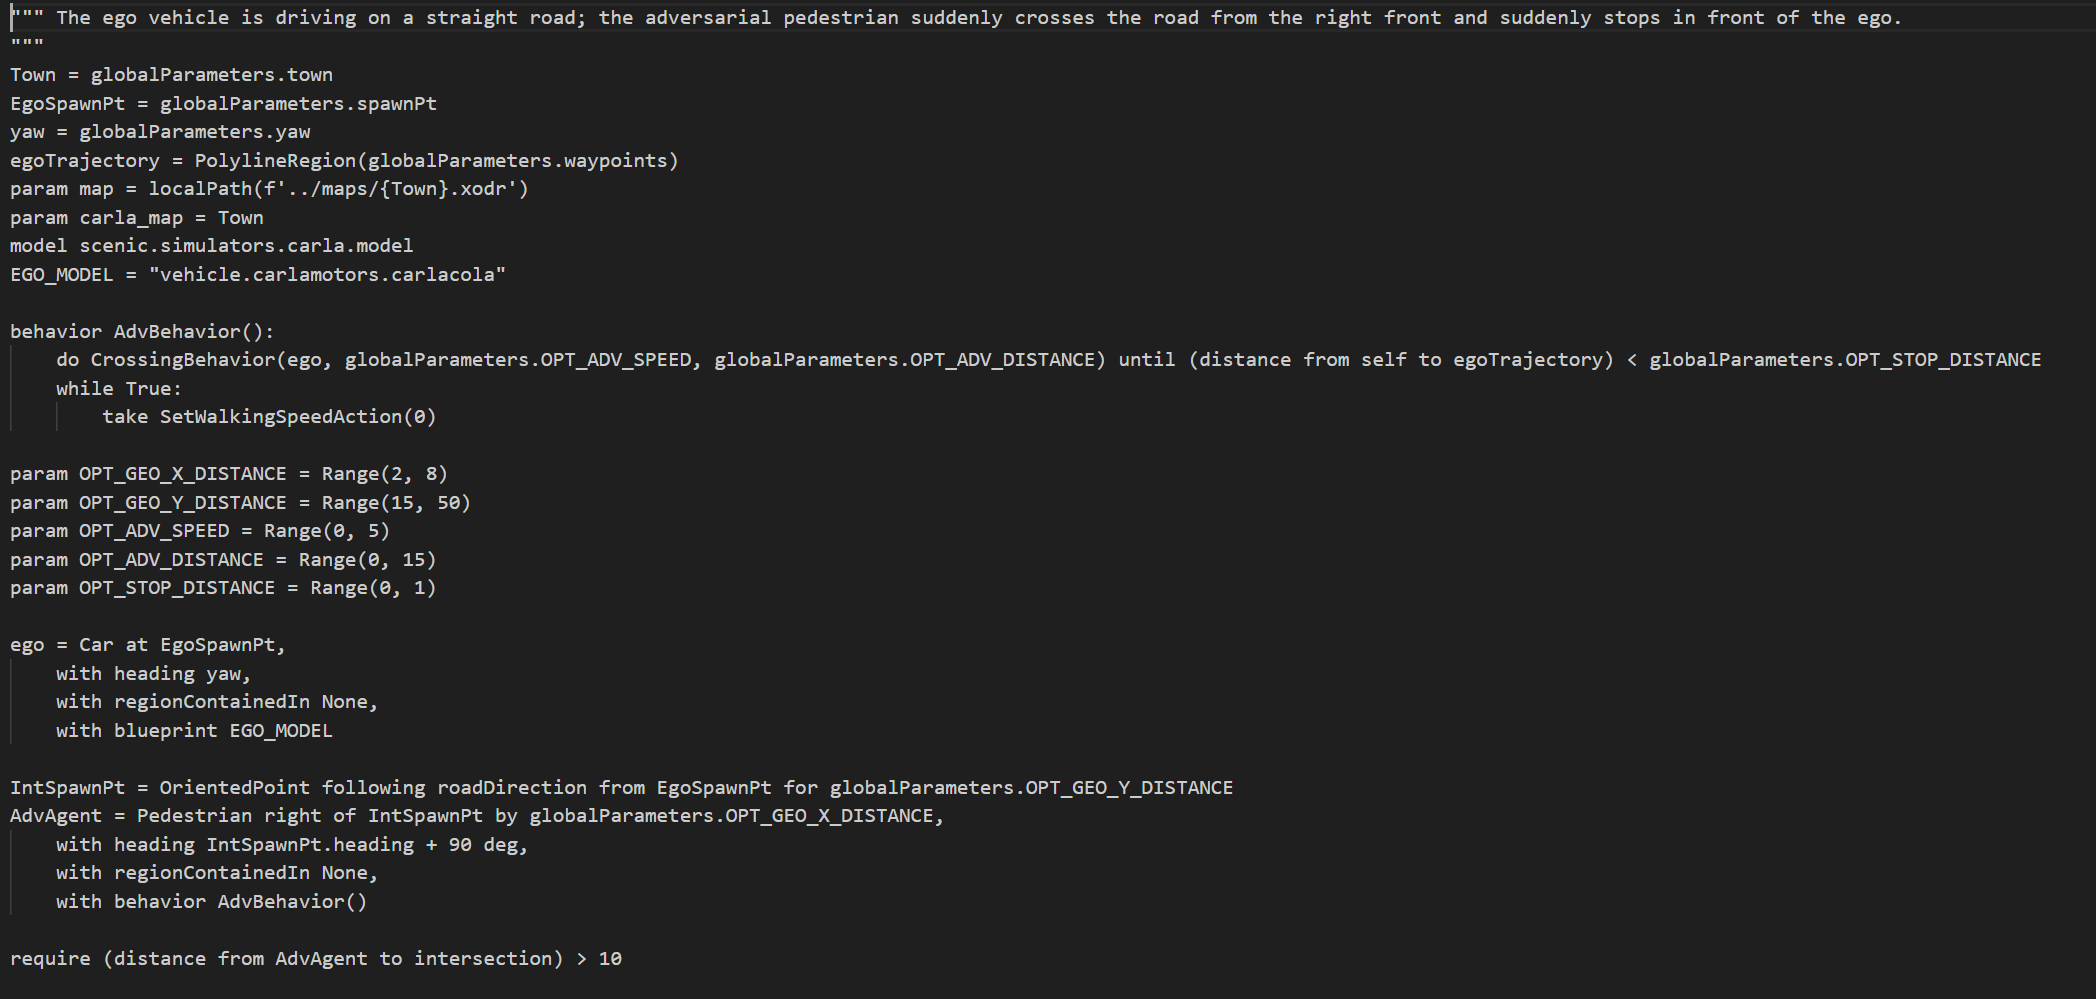
\includegraphics[width=1.0\textwidth]{images/scenic脚本示例1.png}
	\caption{Scenic 脚本示例}
	\label{fig:scenic-example1}
\end{figure}



所示的 Scenic 示例脚本中,系统使用globalParameters模块中的可调参数如
\texttt{OPT\_ADV\\ \_SPEED}、\texttt{OPT\_GEO\_X\_DISTANCE} 等控制行人的行为过程与生成位置,定义的行为函数 \texttt{AdvBehavior()}则包含了先横穿、再停下的动态行为建模。这些参数既可来自模板设定,也可从自然语言推理中注入,最终组合成具有时间逻辑与交互动态的场景剧本。

结构生成模块能够支持在Scenic脚本里添加像位于路口、靠右侧车道这类空间约束以及如距离自车低于一定值停止这种行为触发条件等语义规则,同时系统也支持为多个角色赋予不同行为序列以形成多主体互动的复杂场景。

最终生成的 Scenic 脚本将自动保存至 \texttt{scenario/scenario\_data/scenic\_d\\ata/} 目录下,供后续仿真调度模块调用执行,实现从自然语言到可执行场景的结构化表达闭环。

\subsection{carla仿真模块}

仿真调度模块作为本系统关键组件可实现自动驾驶场景可视化与执行验证,其主要负责把生成的 Scenic 脚本加载到 CARLA 仿真环境里,同时开展仿真初始化、执行控制、传感器采集以及过程管理等工作。该模块在本系统中由封装的 \texttt{ScenicRunnerDynamic} 类实现,调用 Scenic 官方提供的 \texttt{ScenicSimulator} 对生成脚本进行解析,并将其转化为可在 CARLA 中执行的场景实体。

在具体流程方面模块会先读取前一阶段生成的.scenic 脚本,接着通过 Scenic 编译器解析脚本里定义的交通参与者、位置、行为及约束条件,随后系统基于 Carla Python API 建立起仿真连接,配置运行地图、天气参数、物理步长(\texttt{fixed\_delta\_seconds})与同步模式等环境变量。系统默认会采用Carla的同步模式来实施控制,以此保证场景里各参与体的状态更新和传感器采集过程保持一致,进而提升整个仿真过程的稳定性。

在仿真执行过程里系统会自动创建交通参与体像车辆行人等并对其行为轨迹进行初始化,要是Scenic脚本当中定义了行为函数例如行人横穿并在自车前停止等情况,系统就会凭借行为调度逻辑驱动对应实体去执行脚本里预定义的动作,在仿真过程期间模块还会负责记录关键执行信息包含仿真时间对象轨迹碰撞信息交通信号状态等内容,与此同时系统具备截图与视频保存功能能够自动截取仿真中间帧或者生成仿真动画用来进行结果展示与评估。

这个模块的运行过程给系统的“代码,仿真”环节提供了自动化调度能力,并且结合CARLA高保真的渲染与物理驱动能力,为自然语言驱动的场景生成系统提供了可视化反馈与执行验证平台,成为构成系统闭环当中的关键一环。

\subsection{结果评估分析模块}

结果展示模块是系统里用于输出仿真执行结果的重要部分,它能可视化运行过程还可辅助后续评估分析,此模块负责接收来自仿真调度模块的运行数据与视觉信息,并且会以图像视频和行为指标等多种形式呈现生成场景实际效果。

在具体实现的时候系统会在仿真执行进程中调用CARLA所提供的图像传感器接口,自动把关键帧截取下来并保存成静态图片的形式,也能够按照用户的设置把整个仿真过程录制成为视频文件,用来供展示和回放方面使用。与此同时系统支持记录自车以及关键参与体的轨迹坐标相关信息,形成时间序列这种形式的运动轨迹数据,可用于后续的路径可视化或者行车行为评估工作。

run\_eval.py脚本在评估执行方面起着关键作用,是实现场景质量验证和仿真效果分析的重要部分。这个模块以命令行的形式把代理配置文件和场景配置文件作为输入,可自动加载对应的强化学习模型权重,还能调用Scenic与CARLA环境完成整个仿真执行流程。在仿真的过程中,系统会详细记录自车行为和环境交互的数据,涵盖轨迹、速度、加速度以及转向变化等方面的信息,同时会监控碰撞、闯红灯、偏离路线等关键事件。

评估模块集成了一套多维度的指标体系,能够自动计算包含碰撞率、交通违规频率、路线完成度、行为稳定性、舒适性指标和安全性评分的综合性能评估结果。所有的评估数据会统一输出成为日志文件,并且支持以图像或者视频形式记录结果,方便开发者进行回放和可视化分析。系统还内置了自动路径管理机制,确保每轮评估过程的日志和图像结果能够有序存储,有利于进行实验对比和复现。

借助该评估模块,系统能够从自然语言场景生成开始,完整实现仿真、记录、评估的一体化闭环流程,显著提升对生成场景合理性和策略效果的量化验证能力。




